\documentclass{article}
\pagestyle{empty}
\usepackage{amsmath,amssymb,amsfonts}
\usepackage{graphicx}
\usepackage{multicol}
\setlength{\oddsidemargin}{0in} \setlength{\evensidemargin}{0in}
\setlength{\topmargin}{0in} \setlength{\textheight}{8.5in}
\setlength{\textwidth}{6.5in}

\begin{document}
\begin{flushleft}
	\bfseries{MATH 260, Linear Algebra, Spring `14}\\
	\bfseries{Activity 1:  Linear equations and systems, geometrically}\\
	\bfseries{Honor Code:} \hspace{3.5in}\bfseries{Names:}\\
\end{flushleft}
\begin{flushleft}
\vspace{.25in}

Directions:  Everyone should work on the assignment and should fill out their paper.  You are expected to make corrections based on what is presented on the board.  You will NOT turn in the assignment today.  It may be collected in the future.

\vspace{0.2in}

In previous courses you learned about lines and plotting. Today we'll be reviewing a lot of that as a precursor to a more holistic view of systems and LINEar algebra.

\section*{Problem 1:Plotting 2 variables}
\vspace{0.1in}

a) The point-slope form of a line is $y=mx+b$. This is generally easily graphed, most of our equations though will take `standard' form of: $a_1 x + a_2 y = b$. For practice plot the line: $3y-6x=6$.
\vspace{0.1in}
\begin{minipage}{3in}
\includegraphics[scale=0.75]{grid_12_by_12.eps}
\end{minipage}
\vspace{0.2in}

\newpage
b) Now sketch the following pairs of equations:\\
(i) $y=2-4x$ and $y=-4x-3$\\
(ii) $3x+7=y$ and $y=\frac{-2}{3}x-1$\\
(iii) $y=2x+1$ and $3y-3=6x$

\vspace{0.25in}

\begin{minipage}{3in}
\includegraphics[scale=0.75]{grid_12_by_12.eps}
\end{minipage}
\begin{minipage}{3in}
\includegraphics[scale=0.75]{grid_12_by_12.eps}
\end{minipage}
\vspace{0.1in}\\
\begin{minipage}{3in}
\includegraphics[scale=0.75]{grid_12_by_12.eps}
\end{minipage}
\begin{minipage}{3in}
\includegraphics[scale=0.75]{grid_12_by_12.eps}
\end{minipage}

c) When we plot lines, the intersection gives a pair of (x,y) values which will satisfy both equations. How many such pairs do each of the above sets of lines have?\\
\vspace{1in}

Can you draw a pair of lines which has exactly TWO solutions on the fourth grid? Can you come up with any other counts for solutions besides those depicted above?

\newpage
d) Now plot (b-ii) on both of the grids below.\\
(i) On the first also plot $y+1=\frac{-1}{4}x$ \\
(ii) On the second also plot $y=\frac{5}{11}$\\

\vspace{0.2in}

\begin{minipage}{3in}
\includegraphics[scale=.75]{grid_12_by_12.eps}
\end{minipage}
\begin{minipage}{3in}
\includegraphics[scale=.75]{grid_12_by_12.eps}
\end{minipage}
\vspace{0.3in}\\
Similar to having two equations, 3 equations can produce the same types of solution sets: None, one or infinite. Only two of which you've plotted. Notice that we really only needed two equations to get the interesction for (ii), this is called `overdetermined'. Case (i) would be called 'inconsistent' or 'indeterminite'. 

\vspace{0.3in}
\newpage
\section*{Problem 2: Plotting 3 variables}
\vspace{0.1in}
First, actually plotting an equation with 3 variables can be very challenging. We've shown the result below which creates a plane.\\

\begin{minipage}{3in}
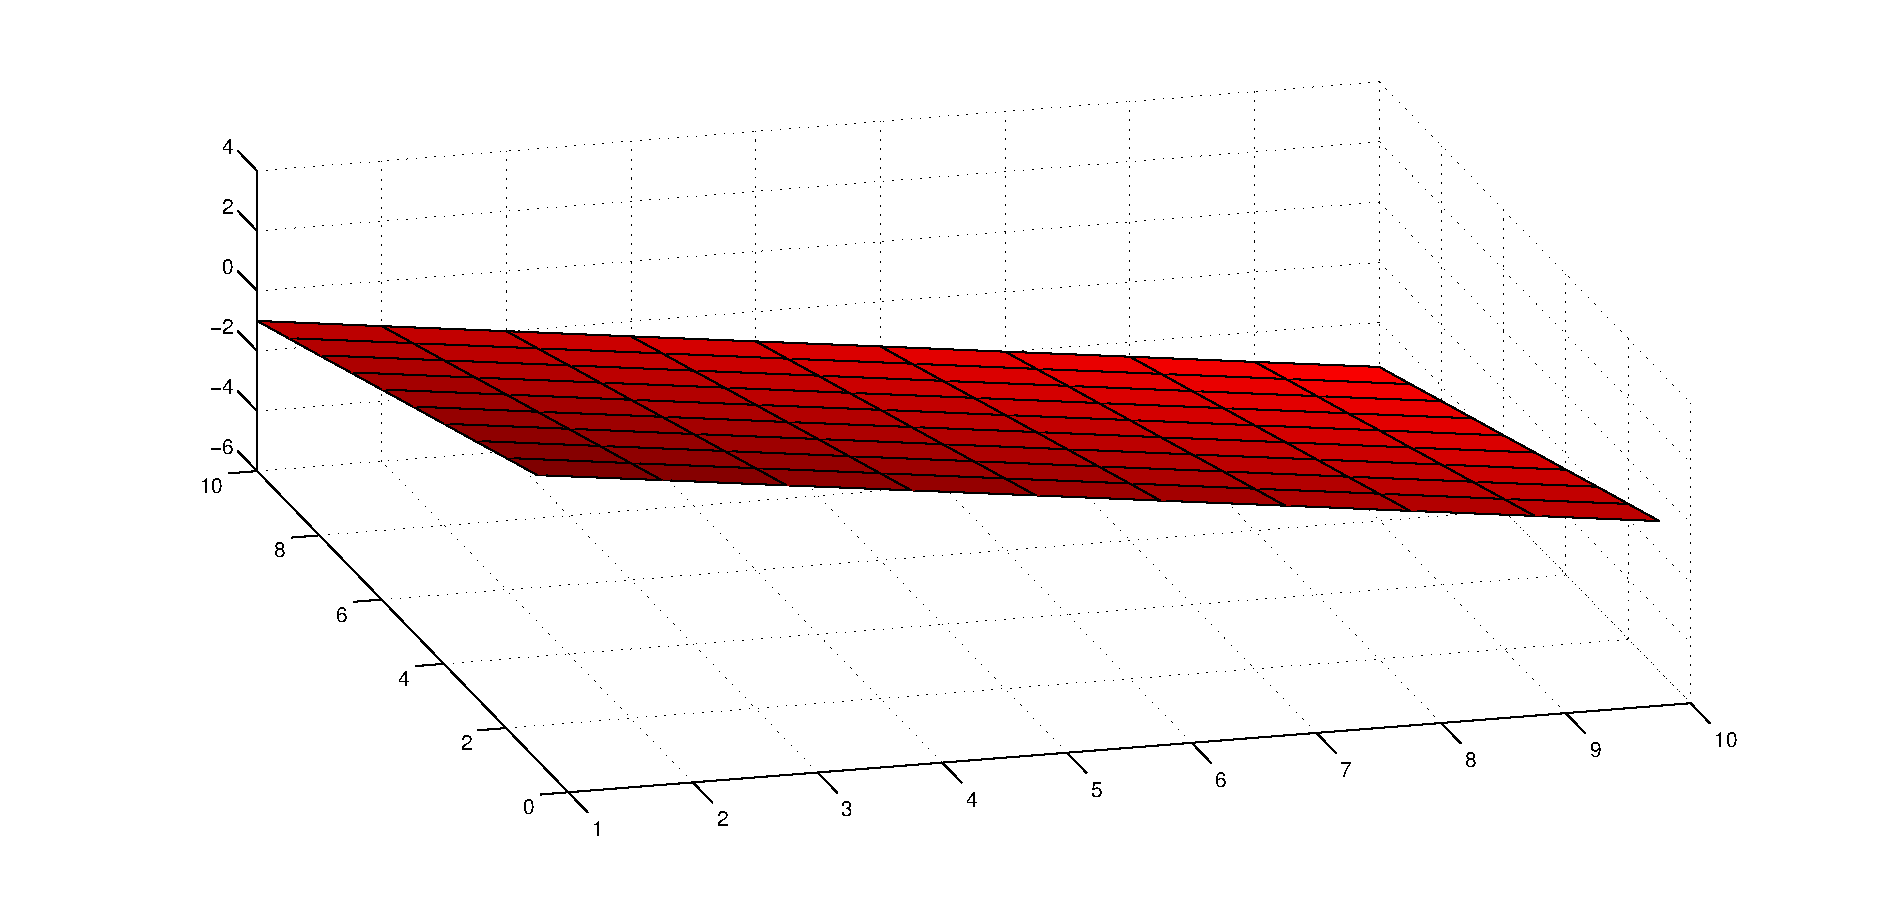
\includegraphics[scale=0.5]{planepic.eps}
\end{minipage}\\
\vspace{0.1in}

Let's look at another system, this time with 3 variables:\\
$x=3z-2y+1$\\
$3z-2y+x=2$\\
Solve this for $x$, $y$, $z$. \textit{Hint: Solve for $z$ first by substituting the first equation into the second}\\
\vspace{1.5in}
Did you get numbers for each variable? What's do you think is going on here? (Feel free to discuss at your table)\\
\vspace{1in}
\Large Notes about this:
\normalsize
\vspace{2in}


\section*{Problem 3}
Time permitting, solve the following systems by elimination:\\

\end{flushleft}
a)
\begin{align*}
x+y&=4\\
x-y&=0
\end{align*}
\vspace{0.1in}

b)
\begin{equation*}
\begin{array}{ccccccr}
x& + &2y&+&z&= &2\\
x& - & y& & &= &4\\
2x&- & y&+&2z&=&0\\
  &  &3y&+& z&=&-2
\end{array}
\end{equation*}

\end{document}